\documentclass{article}
\usepackage[T1]{fontenc}
\usepackage{ae,aecompl}

% Ams math
\usepackage{amsmath}
\usepackage{amssymb}

% Figures
\usepackage{graphicx}

\usepackage{savetrees}

\usepackage{hhline}

\graphicspath{img}


\newcommand{\tref}{t_{\textrm{ref}}}

\begin{document}
\def\oddsBasicSinusoidAmplitudeDecayBasicSinusoid{11.1}
\def\errBasicSinusoidAmplitudeDecayBasicSinusoid{4.3}
\def\oddsBasicSinusoidAmplitudeDecayWithTransientBasicSinusoid{271.9}
\def\errBasicSinusoidAmplitudeDecayWithTransientBasicSinusoid{6.8}
\def\oddsBasicSinusoidAmplitudeDecayBasicSinusoidAmplitudeDecayWithTransient{-260.8}
\def\errBasicSinusoidAmplitudeDecayBasicSinusoidAmplitudeDecayWithTransient{5.8}

\title{Preliminary results on fitting to the AMOC data}
\author{Greg Ashton}
\date{}
\maketitle

In this document we show some preliminary results of fitting phenomological models
to the AMOC data. To select between these phenomological models we will use the
Bayes factor, defined as
\begin{align}
\mathcal{B}(\textrm{model A}, \textrm{model B}) = \frac{P(\textrm{model A}| \textrm{ data})}{P(\textrm{model B}| \textrm{ data})}
\end{align}
such that $\mathcal{B} > 1$ provides evidence for model A over model B, while
$\mathcal{B} < 1$ provides evidence for model B over model A. 

We assume the data is a linear sum of the phenomological model and
gaussian noise to generate a likelihood function for the data. The Bayes factor
is sensitive to both how well the model fits the data, and also the priors chosen
for each model parameter. These priors have been chosen crudely from the data,
and so I will expect the Bayes factors to change when a more expert opinion is
applied.

To fit the models to the data, we have used MCMC simulations which estimate the
posterior distributions for each model parameters. To estimate the marginal
likelihood for each model $P(\textrm{model}| \textrm{ data})$ we have used
so-called `thermodynamic integration', this is a numerical method which has an
associated numerical error which we estimate.

The data that we will consider will be the AMOC flow as a function of the number
of days since the begining of the data set, 2$^{nd}$ April 2004. In the models a
reference time $\tref$ will be used, we set this to the start of the data set
\begin{align}
\tref = \textrm{2}^{nd}\textrm{ April 2004}.
\end{align}

In the following sections we will introduce each model starting with a
base-model , discuss the fit, and then compare between the models.

\section{Basic sinusoidal `base-model'}

First, let us fit a base-model comprising the sum of a linear function and a
sinusoid
\begin{align}
y(t) = y_0 + \dot{y}_0(t - \tref) + A_0 \sin\left(2\pi \frac{t}{P} + \psi_0\right).
\label{eqn: base-model}
\end{align}
This includes all the basic features which are visible by eye in the data.

As we are using a Bayesian methodology, we need to define priors for each of
the model paramters in Eqn.~\eqref{eqn: base-model} and for $\sigma$, the
gaussian noise in the measurements. These are listed in Table~\ref{tab: base-model}
and were chosen from crude estimates to the data. Note that this choice, for the
base-model parameters, will not produce any bias when compared to modifications
since the priors will cancel out. However, modification model parameters could
produce a bias.
\begin{table}[htb]
\centering
\caption{Prior distributions used in the base-model}
\label{tab: base-model}
\begin{tabular}{lll} \hhline{===}
        Parameter & Distribution &  Units\\ \hline
$y_0$ & Unif(\textrm{-}3.0734, 30.8224) & Sv\\
$y_0$ & $\mathcal{N}$(0, ${1.08}\times 10^{\textrm{-}7}$) & Sv/s\\
$A_0$ & Unif(0, 33.8958) & Sv\\
$P$ & Unif(0, 2.0441) & yrs\\
$\psi_0$ & Unif(0, $2\pi$) & rad\\
$\sigma$ & Unif(0, 33.8958) & Sv\\
\hhline{===}
\end{tabular}
\end{table}

In Fig.~\ref{fig: base-model}A we show the posterior distributions of the
base-model model parameters. This demonstrates that the MCMC simulation has
converged to a solution with gaussian posterior values. In Fig.~\ref{fig: base-model}B
we take the maximum posterior estimate, the MCMC sample with the highest posterior
probability, and plot Eqn.~\eqref{eqn: base-model} with these parameters alongside
the original data.
\begin{figure}[htb]
\centering
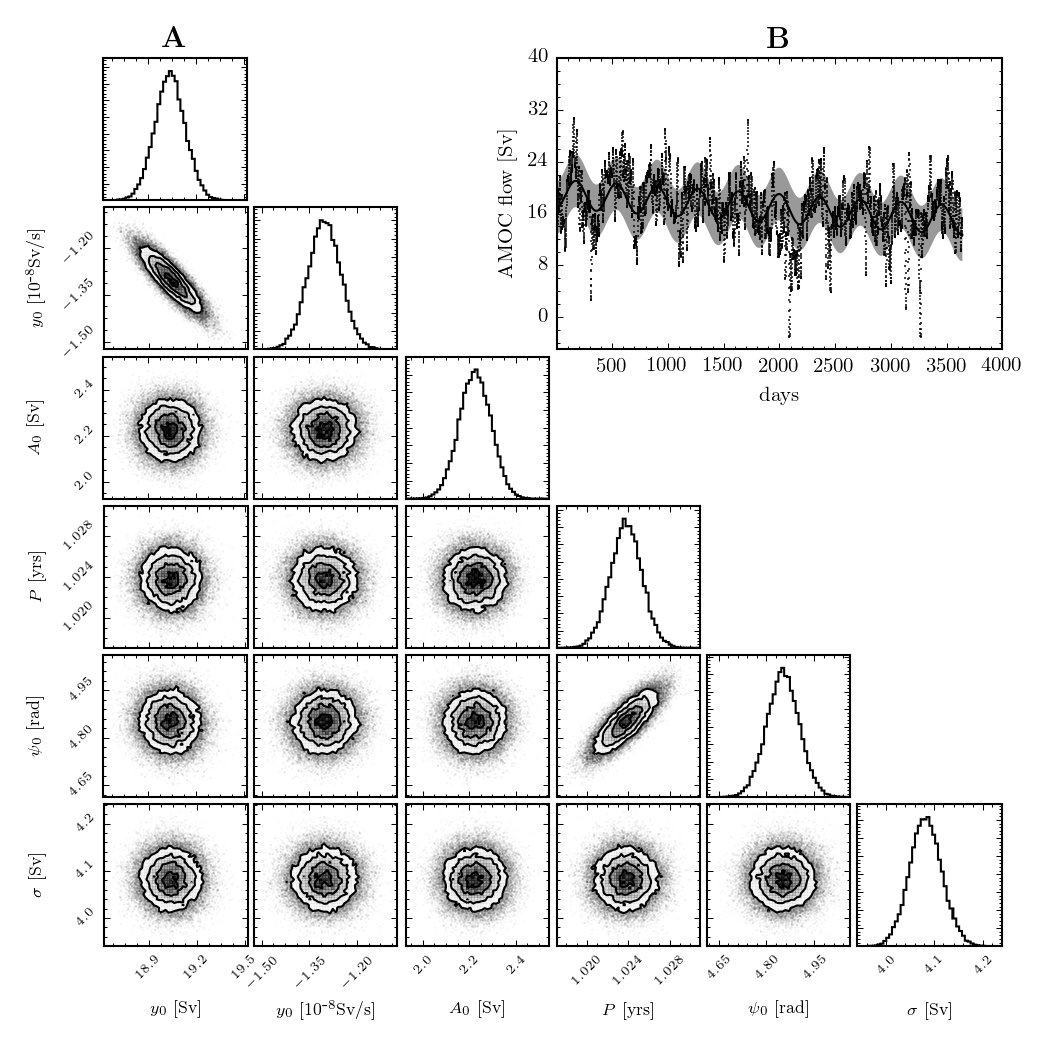
\includegraphics[width=0.8\textwidth]{img/BasicSinusoid_PosteriorWithFit}
\caption{\textbf{A}: Posterior distributions for the model parameters of the
base-model. \textbf{B}: The maximum posterior estimate (MPE) fit to the data.}
\label{fig: base-model}
\end{figure}


\section{Sinusoidal model with evolving amplitude}

The first modification to the base-model we will consider is an evolution of
the sinusoid amplitude.
Specifically, we modify Eqn.~\eqref{eqn: base-model} as follows
\begin{align}
y(t) = y_0 + \dot{y}_0(t - \tref) +
(A_0 + \dot{A}_0(t-\tref)) \sin\left(2\pi \frac{t}{P} + \psi_0\right).
\label{eqn: decay amplitude}
\end{align}
This allows the amplitude to decay $\dot{A} < 0$, or grow $\dot{A} > 0$.

\begin{table}[htb]
\centering
\caption{Prior distributions used in the evolving amplitude model}
\label{tab: base-model}
\begin{tabular}{lll} \hhline{===}
        Parameter & Distribution &  Units\\ \hline
$y_0$ & Unif(\textrm{-}3.0734, 30.8224) & Sv\\
$y_0$ & $\mathcal{N}$(0, ${1.08}\times 10^{\textrm{-}7}$) & Sv/s\\
$A_0$ & Unif(0, 33.8958) & Sv\\
$\dot{A}$ & $\mathcal{N}$(0, ${1.08}\times 10^{\textrm{-}9}$) & Sv/s\\
$P$ & Unif(0, 2.0441) & yrs\\
$\psi_0$ & Unif(0, $2\pi$) & rad\\
$\sigma$ & Unif(0, 33.8958) & Sv\\
\hhline{===}
\end{tabular}
\end{table}

\begin{figure}[htb]
\centering
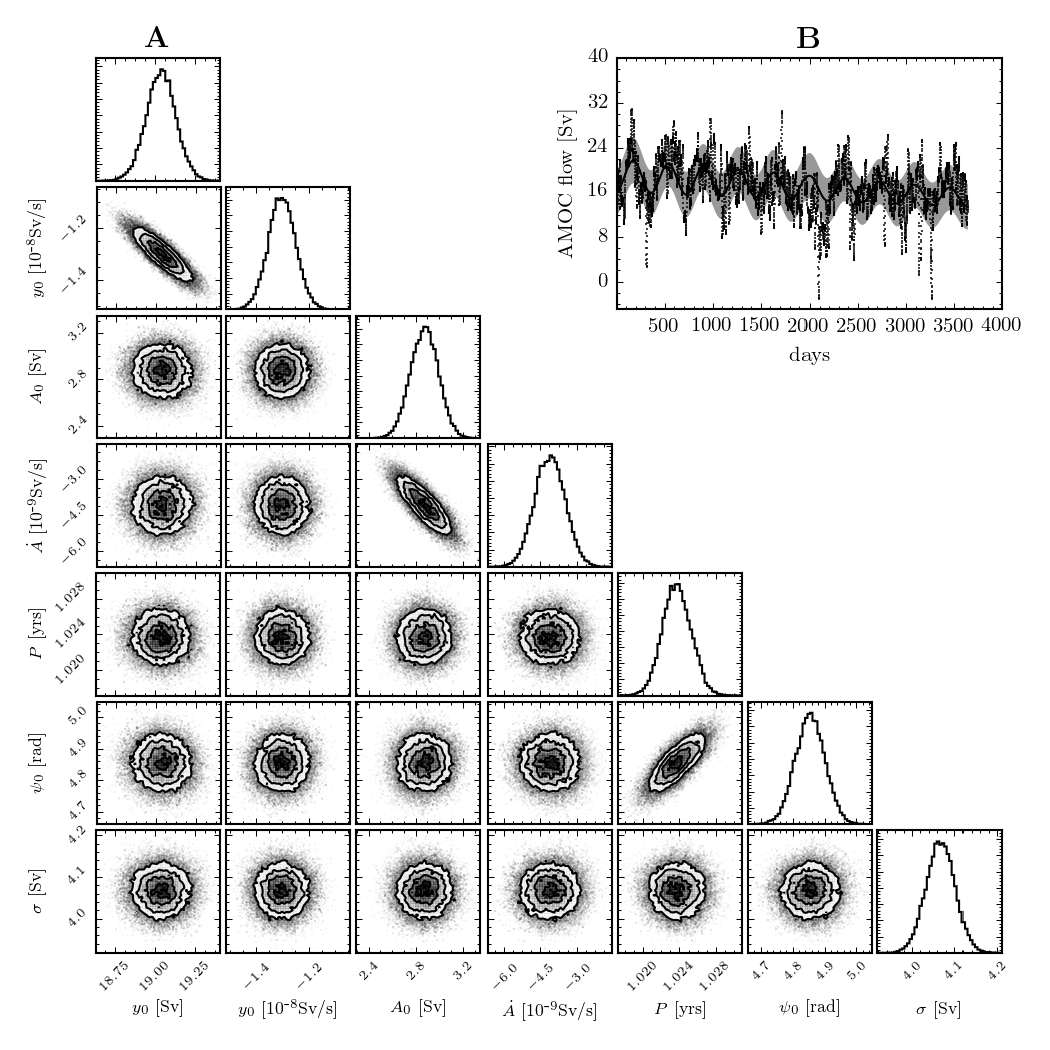
\includegraphics[width=0.8\textwidth]{img/BasicSinusoidAmplitudeDecay_PosteriorWithFit}
\caption{}
\label{fig:}
\end{figure}

\section{Sinusoidal model with amplitude decay and transient}

\begin{align}
y(t) = y_0 + \dot{y}_0(t - \tref) + (A_0 + \dot{A}_0(t-\tref)) \sin\left(2\pi \frac{t}{P} + \psi_0\right)
\end{align}

\begin{table}[htb]
\centering
\caption{Prior distributions used in the evolving amplitude model}
\label{tab: base-model}
\begin{tabular}{lll} \hhline{===}
        Parameter & Distribution &  Units\\ \hline
$y_0$ & Unif(\textrm{-}3.0734, 30.8224) & Sv\\
$y_0$ & $\mathcal{N}$(0, ${1.08}\times 10^{\textrm{-}7}$) & Sv/s\\
$A_0$ & Unif(0, 33.8958) & Sv\\
$\dot{A}$ & $\mathcal{N}$(0, ${1.08}\times 10^{\textrm{-}9}$) & Sv/s\\
$y_1$
 & Unif(0, 33.8958) & Sv\\
$t_1^\mathrm{start}$
 & Unif(0, 3642) & days\\
$t_1^\mathrm{end}$
 & Unif(0, 3642) & days\\
$P$ & Unif(0, 2.0441) & yrs\\
$\psi_0$ & Unif(0, $2\pi$) & rad\\
$\sigma$ & Unif(0, 33.8958) & Sv\\
\hhline{===}
\end{tabular}
\end{table}

\begin{figure}[htb]
\centering
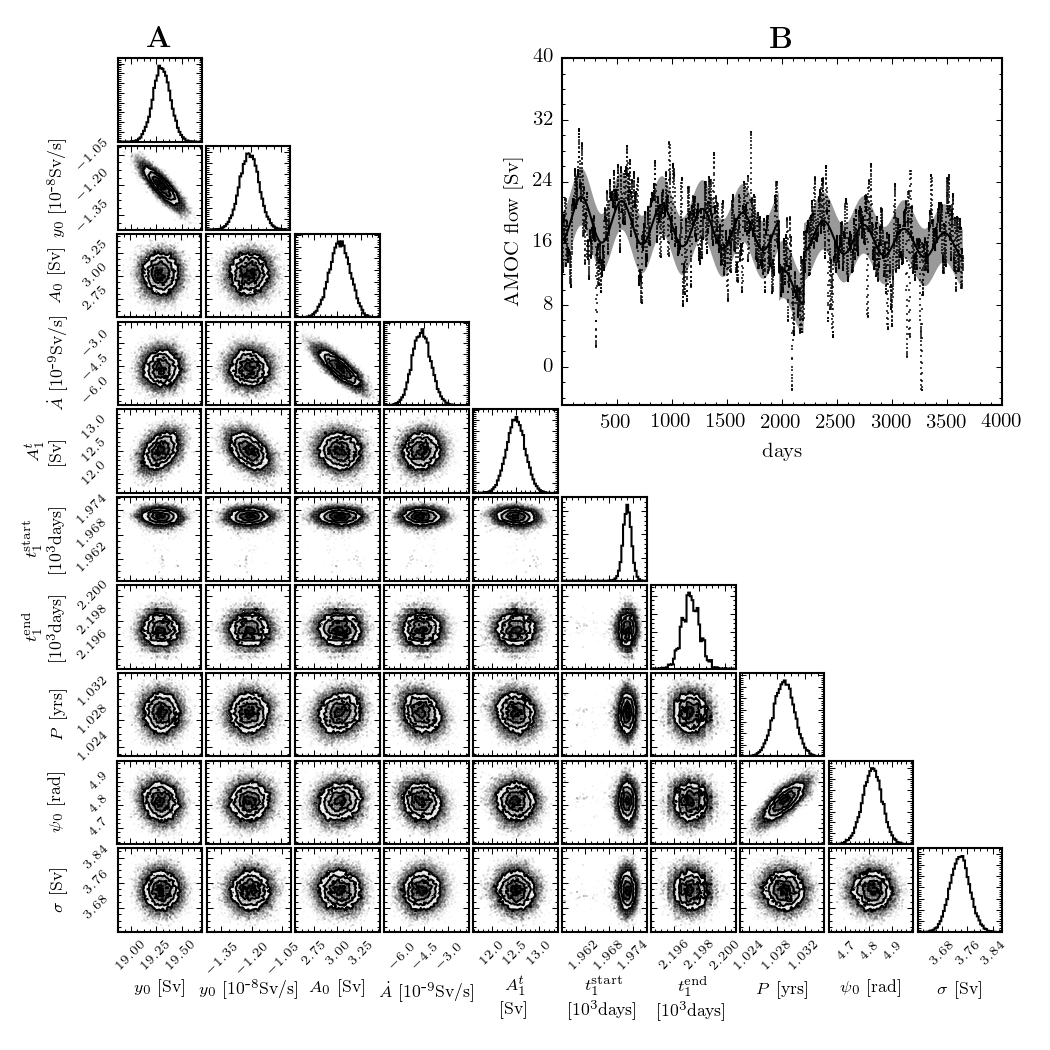
\includegraphics[width=0.8\textwidth]{img/BasicSinusoidAmplitudeDecayWithTransient_PosteriorWithFit}
\caption{}
\label{fig:}
\end{figure}

\section{Bayes factor comparisons}
\begin{table}
\centering
\caption{Bayes factors between the models compared in this work}
\label{}
\begin{tabular}{ccc} \hhline{===}
model A & model B & $\log_{10}(\mathcal{B}(\textrm{model A}, \textrm{model B}))$\\ \hline
evolution of the amplitude & base-model &
$ \oddsBasicSinusoidAmplitudeDecayBasicSinusoid \pm
  \errBasicSinusoidAmplitudeDecayBasicSinusoid$\\
evolution of the amplitude with transient & base-model &
$ \oddsBasicSinusoidAmplitudeDecayWithTransientBasicSinusoid \pm
  \errBasicSinusoidAmplitudeDecayWithTransientBasicSinusoid$ \\
evolution of the amplitude with transient & evolution of the amplitude &
$ \oddsBasicSinusoidAmplitudeDecayWithTransientBasicSinusoidAmplitudeDecay \pm
  \errBasicSinusoidAmplitudeDecayWithTransientBasicSinusoidAmplitudeDecay$
\end{tabular}
\end{table}

\section{Predicting the amplitude decay}





\end{document}
